\documentclass[xetex,table]{beamer}

\usepackage{fontspec}
\usepackage[autostyle]{csquotes}
\usepackage{hyperref}
\usepackage{color}
\usepackage{setspace}
\usepackage{listings}

\usetheme{metropolis}

\title{Elaborazione dati dalla riga di comando}
\author{Luca Ceresoli}
\date{}

\begin{document}

\maketitle

\section{Elaborare dati}

\begin{frame}
  \frametitle{Sistemi per elaborare dati}
  Informatica = elaborazione automatica delle informazioni
  \begin{itemize}
  \item Database relazionali
  \item Spreadsheet
  \item Software ad-hoc
  \item \dots
  \item La riga di comando
  \end{itemize}
\end{frame}

\section{La riga di comando}

\begin{frame}
  \frametitle{La riga di comando}
  \begin{itemize}
  \item Strumento classico, nato ai tempi dai "terminali"
  \item Prompt: richiede un "comando", lo esegue, torna al prompt
  \item Esistono migliaia di possibili comandi
  \item Molto spartana, molto potente
    \begin{itemize}
    \item Presente su praticamente ogni sistema UNIX-like
    \item Utilizzabile su sistemi poco carrozzati...
    \item ...o remoti, con connessioni lentissime
    \end{itemize}
  \end{itemize}
\end{frame}

\begin{frame}
  \frametitle{Standard input, standard output, standard error}
  \begin{center}
    \includegraphics[height=0.6\textheight]{images/process.pdf}
  \end{center}
\end{frame}

\begin{frame}
  \frametitle{Visualizzare i dati}
  \begin{itemize}
  \item \texttt{cat}
  \item \texttt{less}
  \item \texttt{wc}
  \item \texttt{head}, \texttt{tail}
  \item Demo!
  \end{itemize}
\end{frame}

\begin{frame}
  \frametitle{Semplici elaborazioni}
  \begin{itemize}
  \item \texttt{sort}
  \item \texttt{cut}
  \item Demo!
  \end{itemize}
\end{frame}

\section{grep}

\begin{frame}
  \frametitle{grep}
  \begin{itemize}
  \item Filtra le righe, lasciando passare solo le linee che
    corrispondono a un criterio (pattern)
  \item Utilizzo base:
    \begin{itemize}
    \item \texttt{grep {\em PATTERN} file1 file2 file3}
    \item \texttt{grep {\em PATTERN}}
      \begin{itemize}
        \item Filtra lo standard input
      \end{itemize}
    \end{itemize}
  \item Demo!
  \end{itemize}
\end{frame}

\begin{frame}
  \frametitle{grep: varianti}
  \begin{itemize}
  \item Tipi di pattern:
    \begin{itemize}
    \item \texttt{grep {\bf -F} \emph{PATTERN}} --- Ricerca esatta
    \item \texttt{grep {\bf -G} \emph{PATTERN}} --- Basic regular expressions
    \item \texttt{grep {\bf -E} \emph{PATTERN}} --- Extended regular expressions
    \end{itemize}
  \end{itemize}
\end{frame}

\begin{frame}
  \frametitle{grep: opzioni aggiuntive}
  \begin{itemize}
  \item \texttt{-i}: case insentitive
  \item \texttt{-w}: solo parole intere
  \item \texttt{-v}: invert selection: mostra righe {\em non} corrispondenti
  \item \texttt{-l}: mostra solo i nomi dei files corrispondenti
  \item Demo!
  \end{itemize}
\end{frame}

\section{La pipeline}

\begin{frame}
  \frametitle{La pipeline}
  \begin{itemize}
  \item Simbolo: |
  \item Permette di collegare comandi "in catena"
  \item Principio UNIX: ogni software svolge una funzione
    \begin{itemize}
    \item La svolge in modo flessibile ed efficiente
    \item Si integra con altri strumenti che svolgono altre funzioni
    \end{itemize}
  \end{itemize}
\end{frame}

\begin{frame}
  \frametitle{La pipeline}
  Esempio: \texttt{ls -l | grep txt}
  \begin{center}
    \includegraphics[height=0.6\textheight]{images/pipeline.pdf}
  \end{center}
\end{frame}

\section{Usiamo la pipeline}

\begin{frame}
  \frametitle{Semplici elaborazioni}
  \begin{itemize}
  \item \texttt{uniq}
  \item \texttt{tr}
  \item Demo!
  \end{itemize}
\end{frame}

\begin{frame}
  \frametitle{sed}
  \begin{itemize}
  \item sed = the Stream EDitor
  \item Esegue un "programma" formato da coppie pattern (facoltativo)
    + comando
  \item Per ogni riga di input:
    \begin{itemize}
    \item Se il pattern corrisponde, esegue il comando
    \item Altrimenti lascia passare la riga senza modifiche
    \end{itemize}
  \item Comandi principali
    \begin{itemize}
    \item \texttt{s/\emph{regexp}/\emph{replacement}/} --- sostituzione
    \item \texttt{d} --- elimina la riga
    \end{itemize}
  \item Demo!
  \end{itemize}
\end{frame}

\begin{frame}
  \frametitle{awk}
  \begin{itemize}
  \item Struttura simile a \texttt{sed}: coppie pattern + comando
  \item Ma il comando è un vero programma
    \begin{itemize}
    \item linguaggio simile al C
    \end{itemize}
  \end{itemize}
\end{frame}

\begin{frame}
  \frametitle{Grazie per l'attenzione!}

  \begin{center}
    {\Huge Domande?}

    \vspace{0.1\textheight}

    \href{mailto:luca@lucaceresoli.net}{luca@lucaceresoli.net}\\
    \url{http://lucaceresoli.net}

    \textcopyright{} Copyright 2016, Luca Ceresoli\\

    \vspace{0.2\textheight}

    \tiny
    Materiale rilasciato sotto licenza\\
    Creative Commons Attribution - Share Alike 3.0 \\
    \url{https://creativecommons.org/licenses/by-sa/3.0/} \\
\end{center}
\end{frame}

\end{document}
